\documentclass{beamer}
\usetheme{PaloAlto}

\usepackage{graphicx}
\begin{document}
\title{Web-browser based VCD waveform viewer}
\author{Krupa Bathia \\Apurv Mittal \\Rakesh K K}
\institute{Department of Electrical Engineering\\IIT Bombay}
\date{} 
%\frame{\titlepage} 

\frame{\frametitle{Project Objective}
	\begin{itemize}
		\item To create a \textbf{web-browser based VCD waveform viewer} with basic functionalities 
		\begin{itemize}
			\item Displaying the hierarchy
			\item Selecting the signals to be plotted
			\item Viewing the signal transitions
			\item Zoom in/out
			\item Measuring the time difference between the transitions
		\end{itemize} 
		\item Integrate the waveform viewer to Google Chrome
		\item Wishlist
		\begin{itemize}
			\item Integrate the waveform viewer with all the prominent browsers
			\item Load two or more VCDs to compare the waveforms
		\end{itemize}
	\end{itemize}
}

\frame{\frametitle{Project Outline - Tools/Packages and Technology Stack Used}
	\begin{itemize}
		\item Python 2.7.x
		\item SVG (Scalable vector Graphics) file format
		\item Python packages: svgwrite, PyGTK
		\item Google app engine
	\end{itemize}
}

\frame{\frametitle{Outline of work completed}
	\begin{itemize}
		\item A class is defined for VCD file parsing
		\item Class has functions for
			\begin{itemize}
				\item Listing the signals with the hierarchy information
				\item Extracting the transitions of the signals and then saving in a dictionary
				\item Given two timestamps and a signal list, all the transitions of each signal in the list between the timestamps are returned
				\item Listing the values of the signals at a particular time instant
			\end{itemize}
		\item Frontend of the project: started with Google app builder
	\end{itemize}
}

\frame{\frametitle{Outline of the work to be done}
	\begin{itemize}
		\item Representing data in SVG format
		\item Integrating the SVG file in the app using python
		\item To make the GUI and integrate it with the browser
	\end{itemize}
	\begin{figure}[htp]
\centering
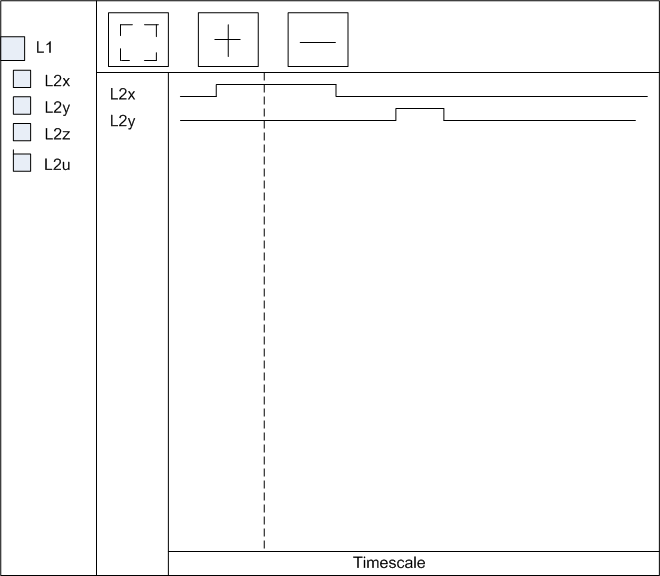
\includegraphics[scale=0.30]{barvcdviewer.png}
%\caption{VCD viewer}
\label{}
\end{figure}
}

\end{document}